% This is the chapter 'Modeling' to the "Hodgkin-Huxley neuron model V2.0 book"
% Last edited 2026.08.08


\chapter[Thermodynamic model]{Thermodynamic model\label{ch:V2-0Modell-Thermodynamic}}

\iflatexml
\else
\minitoc
\fi


The experience that not only electrical but also thermodynamic (temperature) changes occur in the neuron during the action potential is practically the same age as the observation of electrical phenomena. Later, with the development of measurement techniques, other phenomena (force effects, pressure waves, optical and density changes, etc.) were also observed. These phenomena cannot be explained by the single-discipline V1.0 theory, although they are perfectly consistent with the electrical effect and their time course is also the same; see figure~\ref{fig:HHGradient}.

As Hodgkin wrote: "Hill and his colleagues found~\cite{HeatProductionNeuron:1958} that an initial phase of heat liberation [of the \gls{AP}] was followed by one of
heat absorption. [...] a net cooling on open-circuit was totally unexpected
and has so far received no satisfactory explanation."~\cite{HodgkinConduction:1964}
"All authors came to similar conclusions: during
the \gls{AP}, \textit{no significant net heat is produced}. Transient heat releases are mostly reabsorbed in the second phase of the \gls{AP}. \dots The finding of a reversible heat release during the action potential of
nerves is a striking and very fundamental fact. It is inconsistent with the
\gls{HH} model.
The physics underlying the nervous impulse
must rather be based on reversible processes".~\cite{ThermalBiophysics:2007}


\begin{figure}
\centering
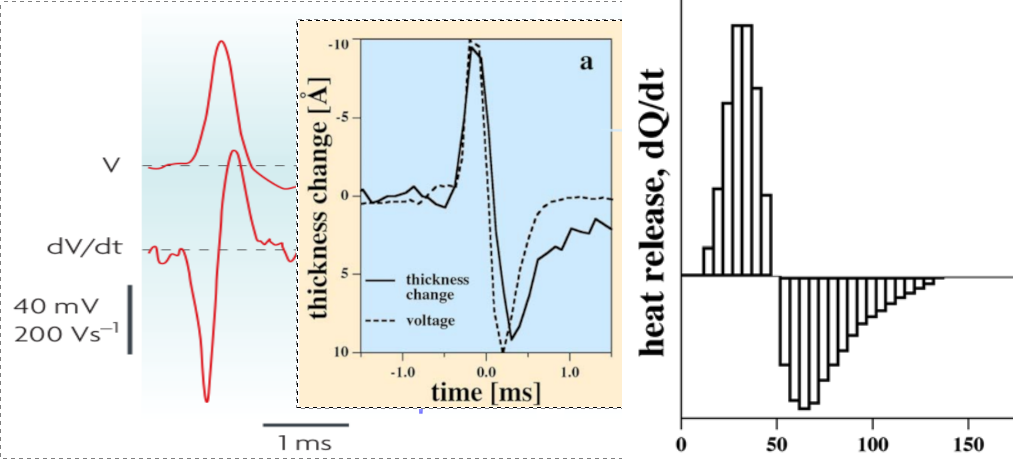
\includegraphics[width=.85\textwidth]{fig/ElasticityGradientHeimburg.png}
\caption{\label{fig:HHGradient}
The time course of the electric gradient perfectly matches that of the mechanical and thermal changes; however, classic theory cannot explain the connection between them~\cite{HeimburgPhysikOfNerves:2009}. See Fig. ?? how the phase diagram of the voltage change in the function of its gradient matches the experimentally measured values.}	
\end{figure}

\ifx\magyar\undefined  
\section[The neuron as a Carnot-engine]{The neuron as Carnot-engine\label{sec:Model-CarnotEngine}}
\else
\subsection[A neuron mint Carnot-gép]{A neuron mint Carnot-gép\label{sec:Model-CarnotEngine}}
\fi

\ifx\magyar\undefined  
In simple words, a neuron combines different disciplines; it works like a two-tact biological internal combustion engine, and can be described theoretically as a special Carnot-type thermodynamic engine, see section~\ref{sec:Physics-Thermodynamics}. The synaptic input currents operate the ignition. The influx of $Na^+$ ions acts like an explosion, producing a large pressure impulse due to electrical repulsion between ions; see section~\ref{sec:Physics-Speculations}. The neuron's volume remains practically unchanged (representing an iso-volume process), and the pressure wave vibrates the particles (including dissociated ions) as a longitudinal wave, and the resulting offset potential moves the ions out of the neuron through the only available output channel: the axon. The pressure wave is similar to a sound wave, with negligible material transport. 
The force analysis shows that the pressure wave
causes a longitudinal vibration, while the changed potential adds
a potential-dependent longitudinal force component for moving the ions.
\else
Egyszerűen fogalmazva, a neuron több fizikai diszciplinát kombinál össze.
Úgy működik, mint egy két-ütemű biológiai belső égésű motor,
és elméletileg egy speciális Carnot-féle termodinamikai gépnek
tekinthető.
A szinaptikus bemenő áram gyújtásként hat. A $Na^+$ ionok rendkívül gyors beáramlása robbanásként hat,
és nagy nyomás- és feszültség-gradienst hoz létre.
A neuron térfogata gyakorlatilag változatlan marad (azonos térfogatú folyamat),
és a nyomáshullám rezgeti a részecskéket (köztük a disszociált ionokat) longitudinális hullámként,
a keletkezett többlet potenciál pedig mozgatja az ionokat az egyetlen lehetséges  kilépési útvonal: az axon felé. 
A nyomáshullám egy hanghullámhoz hasonló, elhanyagolható anyagszállítással.
Az erők analízise azt mutatja, hogy a nyomáshullám longitudinális rengést okoz, a megváltozott potenciál pedig egy longitudinális 
erőkomponenssel járul hozzá az ion mozgatásához.
\fi


\ifx\magyar\undefined
The two-tact engine, in the first stroke, the pressure impulse invests energy into compressing the elastic membrane and starting a compression wave (a soliton). In the first tact, the elastic membrane pumps out some electrolyte, and in the second tact it pumps in part of the electrolyte (the driving force is a combined thermoelectrical/mechanical force rather than some magic battery). The pumping goes through the ion channels in the \gls{AIS}, which "resists" it, thereby generating a potential wave known as \gls{AP}; well described by electricity. The force analysis shows that the pressure wave
causes a longitudinal vibration, while the changed potential adds
a potential-dependent longitudinal force component for moving the ions. Compressing the electrolyte
produces heat, as evidenced by a rise in temperature. The expansion consumes heat, as evidenced by a decrease in temperature. These are well-understood processes in thermodynamics.
However, they are still unexplained in biophysics, although they were observed
seven decades ago~\cite{HeatProductionNeuron:1958}.
The elastic membrane functions as a damped oscillator, which, in its negative amplitude phase, reverses the direction of electrolyte flow (and, consequently, the direction of the current carried by the ions).
In the discipline of electricity (when using the serial $RC$ model), it can be interpreted as a capacitive current, which in physiology is observed as hyperpolarization that inverts the polarity of the output voltage.
The ions represent both mass and charge simultaneously, and, correspondingly, one can observe, in addition to the electrical potential wave, mechanical, optical, and other features changing.
In different disciplines, pressure and voltage represent the same phenomenon, using concepts from various disciplines.
Both waves propagate with the speed of the carrier.

\else
A kétütemű motor működésének első ütemében a nyomás erőlökése
energiát fordít a  rugalmas membrán összenyomásába és elindít 
egy nyomáshullámot (soliton).
Az első ütemben a rugalmas membrán elektrolitot pumpál ki
az \gls{AIS} ioncsatornáin keresztül, a második ütemben pedig részben visszaszívja azt. A csatornák "ellenállnak",
ezért az \gls{AP} néven ismert potenciálhullámot hozzák létre;
a jelenséget az elektromosságtan jól leírja. 
(a hajtóerő tehát egy kombinált termodinamikai/elektromos erő,
és nem valamiféle állandó vagy mágikusan változó  feszültségű
feszültséggenerátor)
A folyadék összenyomása hőt termel, ami hőmérséklet emelkedésben 
nyilvánul meg.
A kiterjedés hőt fogyaszt, ami hőmérséklet csökkenésben nyilvánul meg.
A termodinamikában ezek jól ismert folyamatok, 
de a biofizika annak ellenére nem tudja magyarázni, hogy a folyamatokat
már hét évtizeddel ezelőtt megfigyelték.~\cite{HeatProductionNeuron:1958}.
A rugalmas membrán egy csillapított oszcillátorként működik,
ami, a negatív amplitúdójú fázisban, megfordítja az elektrolite folyadék
áramlásának irányát (beleértve a szállított ionok áramlásának irányát is).
Ez a jelenség az elektromosságtanban (amikor soros  $RC$  modellt használjuk), kapacitív áramként értelmezhető, amit a fiziológia 
hiperpolarizációként figyel meg, ami megfordítja a kimenő feszültség polaritását.
Az ionok egyidejűleg jelentenek tömeget és töltést,
és ennek megfelelően, az elektromos potenciál hullám mellett,
mechanikai, optikai és egyéb tulajdonságok is változnak. 
A különböző diszciplinákban a nyomás és a feszültség 
ugyanazt a jelenséget mutatják a megfelelő diszciplina saját
fogalmai szerint, amit az is alátámaszt, hogy mindkét hullám a hordozó sebességével terjed.

\fi

\ifx\magyar\undefined
\section{Heat emission/absorption\label{sec:HeatAbsorption}}
\else
\section{Hőkibocsátás és elnyelés\label{sec:HeatAbsorption}}
\fi

\ifx\magyar\undefined
The early experimental observation~\cite{HeatProductionNeuron:1958}, that positive and negative heat production is associated with a nerve impulse, suggested a thermodynamic model. 
In the framework of the classical
theory, Ohmic currents flow through resistors that dissipate heat due to
friction, no matter in which direction ($W=I^2\times R$) the ion currents flow.
The existence of "cooling", alone, undermines the credibility of the classic theory~\cite{HEIMBURGReversibleHeatProduction:2021}.
The issue here is that the dissipation was attributed to the "leakage current."  
As Hodgkin wrote: "Hill and his colleagues found~\cite{HeatProductionNeuron:1958} that an initial phase of heat liberation [of the action potential] was followed by one of
heat absorption. [...] a net cooling on open-circuit was totally unexpected
and has so far received no satisfactory explanation."~\cite{HodgkinConduction:1964}
"All authors came to similar conclusions: during
the action potential, no significant net heat is produced. Transient heat releases are mostly reabsorbed in the second phase of the action potential. \dots The finding of a reversible heat release during the action potential of
nerves is a striking and very fundamental fact. It is inconsistent with the
\gls{HH} model. The physics underlying the nervous impulse
must rather be based on reversible processes".~\cite{ThermalBiophysics:2007} 
At that time it was commonly known that compressing a
medium produces heating and extending it causes cooling.
Although modeling neuron as a thermodynamic engine 
that is heated and cooled, and produced no significant net heat, would be trivial, no such model came to light.
The probable reason is that no reasonable idea
shined up that could attach the observed heat absorbtion
with the observed evident signs of the electrical operations.

\else

\fi


\ifx\magyar\undefined

Heat liberation and absorption are direct experimental evidence of the "slow current" and the mechanisms described above.
The lack of leakage current
not only validates our model, but also solves the long-standing mystery of reversible heat release during the \gls{AP}.
Pressure changes accompany the electrical process and naturally account for the observed temperature changes.
The energy consumption of the nervous impulse underpins that the complex physical process comprises mostly reversible disciplinary processes:
most of the energy of \gls{AP} is stored as reversible elastic potential energy. Hence, its dissipation is also negligible: "no significant net heat is produced"~\cite{ThermalBiophysics:2007}. 

The shocking conclusion in~\cite{MechanicalBrainPulses:2018}, that "brain cells communicate
with mechanical pulses, not electrical signals", more precisely sounds
that the elastic membrane generates a pressure wave in the volume of the 
membrane, and all components having mass (the electrolyte) vibrate "in place". The charged components (the ions, a $10^{-3}$ part of the electrolyte) repel each other (as long as there is excess charge on the membrane) toward the \gls{AIS} and along the membrane.
Actually, the disciplines of thermodynamics and electricity cooperate in both producing and transmitting \gls{AP}. Neither of them can do that alone. No compromise is needed.
The nervous pulse transmission over the axons 
also must be revisited. The classical mechanism based on coordinated action
of ion channels is undoubtedly wrong. Among others, the physical conditions of applicability of the telegrapher's equations are not fulfilled, plus (see Appendix~\ref{sec:Forces}) the electrical forces are orders of magnitude weaker than the elastic ones. The enormous pressure, the incompressible electrical fluid,
and the repulsion of the delivered particles suggest 
an alternative and more reasonable mechanism.
The resultant of the electrical and thermodynamic, and first of all, the mechanical force generated by the elastic membrane, does the task.
No protein mechanisms and cooperating ion channels are needed.

\else

\fi
